\documentclass[12pt, a4paper]{ctexart}
\usepackage[margin=2.2cm]{geometry}
\usepackage{amsmath, amssymb}
\usepackage{enumitem}
\usepackage{tcolorbox}
\usepackage{booktabs}
\usepackage{array}
\usepackage{fancyhdr}
\usepackage{xcolor}
\usepackage{tikz}
\usepackage{hyperref}
\usepackage{graphicx}
\usepackage{multirow}

% 颜色定义
\definecolor{mainblue}{RGB}{41, 98, 168}
\definecolor{lightblue}{RGB}{230, 240, 255}
\definecolor{tipgreen}{RGB}{34, 139, 87}
\definecolor{lightgreen}{RGB}{235, 250, 240}
\definecolor{warnred}{RGB}{200, 50, 50}
\definecolor{lightred}{RGB}{255, 240, 240}
\definecolor{examorange}{RGB}{210, 120, 20}
\definecolor{lightorange}{RGB}{255, 248, 235}
\definecolor{apppurple}{RGB}{120, 60, 170}
\definecolor{lightpurple}{RGB}{245, 238, 255}

% 页眉页脚
\pagestyle{fancy}
\fancyhf{}
\fancyhead[L]{\small\textcolor{mainblue}{\textbf{人教版八年级下册 · 第17章}}}
\fancyhead[R]{\small\textcolor{mainblue}{勾股定理讲义}}
\fancyfoot[C]{\small —\ \thepage\ —}
\renewcommand{\headrulewidth}{0.6pt}
\renewcommand{\headrule}{\hbox to\headwidth{\color{mainblue}\leaders\hrule height \headrulewidth\hfill}}
\renewcommand{\footrulewidth}{0pt}

% tcolorbox 样式
\newtcolorbox{knowledgebox}[1][]{
  colback=lightblue, colframe=mainblue,
  fonttitle=\bfseries\large, title=#1,
  arc=3mm, boxrule=0.8pt,
  left=8pt, right=8pt, top=6pt, bottom=6pt
}

\newtcolorbox{tipbox}[1][]{
  colback=lightgreen, colframe=tipgreen,
  fonttitle=\bfseries, title=#1,
  arc=2mm, boxrule=0.6pt,
  left=6pt, right=6pt, top=4pt, bottom=4pt
}

\newtcolorbox{warnbox}[1][]{
  colback=lightred, colframe=warnred,
  fonttitle=\bfseries, title=#1,
  arc=2mm, boxrule=0.6pt,
  left=6pt, right=6pt, top=4pt, bottom=4pt
}

\newtcolorbox{examplebox}[1][]{
  colback=lightorange, colframe=examorange,
  fonttitle=\bfseries, title=#1,
  arc=3mm, boxrule=0.8pt,
  left=8pt, right=8pt, top=6pt, bottom=6pt
}

\newtcolorbox{appbox}[1][]{
  colback=lightpurple, colframe=apppurple,
  fonttitle=\bfseries, title=#1,
  arc=3mm, boxrule=0.8pt,
  left=8pt, right=8pt, top=6pt, bottom=6pt
}

\setCJKmainfont{Hiragino Sans GB}
\setCJKsansfont{Heiti SC}

\begin{document}

% ============ 标题页 ============
\begin{center}
{\Huge\bfseries\textcolor{mainblue}{第17章\quad 勾股定理}}\\[12pt]
{\Large\textcolor{gray}{讲\quad 义}}\\[8pt]
\rule{0.6\textwidth}{1pt}\\[8pt]
{\normalsize 适用：人教版\quad 八年级下册\quad |\quad 课时：2课时（90分钟）}
\end{center}
\vspace{10pt}

% ============ 第一部分：知识点讲解 ============
\section*{\textcolor{mainblue}{一、知识点讲解}}

\subsection*{1.1\quad 勾股定理}

\begin{knowledgebox}[定理内容]
如果直角三角形的两条直角边分别为 $a$、$b$，斜边为 $c$，那么
\[
\boxed{a^2 + b^2 = c^2}
\]
\end{knowledgebox}

\vspace{6pt}

\textbf{几何理解：}

\begin{center}
\begin{tikzpicture}[scale=1.2]
  \coordinate (A) at (0,0);
  \coordinate (B) at (3,0);
  \coordinate (C) at (3,2);
  \draw[thick, mainblue] (A)--(B)--(C)--cycle;
  \draw[fill=mainblue!15] (2.7,0) rectangle (3,0.3);
  \node[below] at (1.5,0) {$a$};
  \node[right] at (3,1) {$b$};
  \node[above left] at (1.5,1) {$c$（斜边）};
\end{tikzpicture}
\end{center}

\begin{itemize}[leftmargin=2em]
  \item 直角所对的边叫\textbf{斜边}（最长的边），记为 $c$
  \item 另外两条边叫\textbf{直角边}，分别记为 $a$、$b$
  \item 文字表述：\textbf{两条直角边的平方和等于斜边的平方}
\end{itemize}

\begin{warnbox}[易错提醒]
\begin{itemize}[leftmargin=1.5em, itemsep=2pt]
  \item 斜边一定是 $c$，不能搞混！只有 $c$ 在等号右边时公式才是 $a^2+b^2=c^2$
  \item 勾股定理\textbf{只适用于直角三角形}
\end{itemize}
\end{warnbox}

\subsection*{1.2\quad 勾股定理的逆定理}

\begin{knowledgebox}[逆定理]
如果三角形的三边 $a$、$b$、$c$ 满足 $a^2 + b^2 = c^2$，那么这个三角形是\textbf{直角三角形}，且 $c$ 所对的角是直角。
\end{knowledgebox}

\vspace{4pt}

\begin{center}
\renewcommand{\arraystretch}{1.4}
\begin{tabular}{|c|c|c|}
\hline
 & \textbf{正定理} & \textbf{逆定理} \\
\hline
\textbf{条件} & 已知是直角三角形 & 已知三边长度 \\
\hline
\textbf{结论} & 求边长 & 判断是否为直角三角形 \\
\hline
\end{tabular}
\end{center}

\subsection*{1.3\quad 常见勾股数组}

满足 $a^2+b^2=c^2$ 的\textbf{正整数}组合叫勾股数：

\begin{center}
\renewcommand{\arraystretch}{1.3}
\begin{tabular}{|c|c|}
\hline
\textbf{勾股数} & \textbf{验证} \\
\hline
3,\ 4,\ 5 & $9+16=25$ \\
\hline
5,\ 12,\ 13 & $25+144=169$ \\
\hline
6,\ 8,\ 10 & $36+64=100$\quad（3,4,5 的 2 倍） \\
\hline
8,\ 15,\ 17 & $64+225=289$ \\
\hline
7,\ 24,\ 25 & $49+576=625$ \\
\hline
\end{tabular}
\end{center}

\begin{tipbox}[规律]
一组勾股数同时乘以同一个正整数 $k$，得到的仍然是勾股数。\\
例如：$3,4,5 \;\to\; 6,8,10 \;\to\; 9,12,15 \;\to\; \cdots$
\end{tipbox}

% ============ 第二部分：例题精讲 ============
\section*{\textcolor{examorange}{二、例题精讲}}

% --- 例题1 ---
\begin{examplebox}[【例题1】已知直角三角形两边，求第三边]
\textbf{题目：}在直角三角形中，\\
（1）已知两直角边 $a=6$，$b=8$，求斜边 $c$；\\
（2）已知一直角边 $a=5$，斜边 $c=13$，求另一直角边 $b$。

\vspace{6pt}
\textbf{解答：}

（1）由勾股定理：
\[
c^2 = a^2 + b^2 = 6^2 + 8^2 = 36 + 64 = 100 \implies c = \sqrt{100} = \boxed{10}
\]

（2）由勾股定理：
\[
b^2 = c^2 - a^2 = 13^2 - 5^2 = 169 - 25 = 144 \implies b = \sqrt{144} = \boxed{12}
\]
\end{examplebox}

\begin{tipbox}[方法总结]
\begin{itemize}[leftmargin=1.5em, itemsep=2pt]
  \item 求斜边：$c = \sqrt{a^2 + b^2}$（两直角边平方和开方）
  \item 求直角边：$a = \sqrt{c^2 - b^2}$（斜边平方减去另一条直角边的平方再开方）
\end{itemize}
\end{tipbox}

% --- 例题2 ---
\begin{examplebox}[【例题2】判断三角形是否为直角三角形]
\textbf{题目：}判断以下各组边长能否构成直角三角形：\\
（1）$a=7$，$b=24$，$c=25$ \qquad
（2）$a=4$，$b=5$，$c=6$

\vspace{6pt}
\textbf{解答：}

（1）最大边 $c=25$，验证：
\[
a^2 + b^2 = 7^2 + 24^2 = 49 + 576 = 625 = 25^2 = c^2
\]
$\because\; a^2+b^2=c^2$，$\therefore$ 是直角三角形。\quad $\checkmark$

\vspace{4pt}
（2）最大边 $c=6$，验证：
\[
a^2 + b^2 = 4^2 + 5^2 = 16 + 25 = 41 \neq 36 = c^2
\]
$\because\; a^2+b^2 \neq c^2$，$\therefore$ 不是直角三角形。\quad $\times$
\end{examplebox}

\begin{tipbox}[方法总结]
\begin{enumerate}[leftmargin=1.5em, itemsep=2pt]
  \item 找出最长边 $c$
  \item 计算两条较短边的平方和，与最长边的平方比较
  \item 相等 $\to$ 直角三角形；不相等 $\to$ 不是
\end{enumerate}
\end{tipbox}

% --- 例题3 ---
\begin{examplebox}[【例题3】勾股定理与坐标系结合]
\textbf{题目：}在平面直角坐标系中，点 $A(0,0)$，点 $B(3,4)$，求 $AB$ 的长度。

\vspace{6pt}
\textbf{解答：}

过点 $B$ 向 $x$ 轴作垂线，垂足为 $C(3,0)$。\\
在直角三角形 $ACB$ 中：
\[
AC = 3,\quad BC = 4,\quad AB \text{ 为斜边}
\]
\[
AB = \sqrt{AC^2 + BC^2} = \sqrt{3^2 + 4^2} = \sqrt{9+16} = \sqrt{25} = \boxed{5}
\]
\end{examplebox}

\begin{tipbox}[引申公式——两点间距离公式]
两点 $(x_1,y_1)$ 和 $(x_2,y_2)$ 之间的距离：
\[
d = \sqrt{(x_2 - x_1)^2 + (y_2 - y_1)^2}
\]
\end{tipbox}

% --- 例题4 ---
\begin{examplebox}[【例题4】折叠与勾股定理（方程思想）]
\textbf{题目：}长方形 $ABCD$ 中，$AB=8$，$BC=6$。将 $\triangle ABE$ 沿 $BE$ 折叠，使点 $A$ 落在 $A'$ 处，且 $A'$ 恰好在对角线 $BD$ 上。求 $AE$ 的长度。

\begin{center}
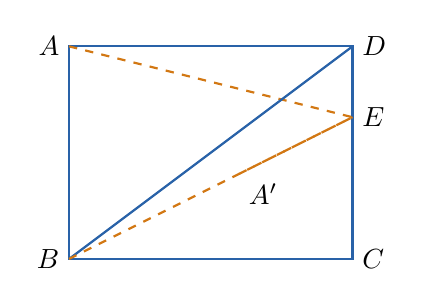
\begin{tikzpicture}[scale=0.9]
  \coordinate (A) at (0,3);
  \coordinate (B) at (0,0);
  \coordinate (C) at (4,0);
  \coordinate (D) at (4,3);
  \coordinate (E) at (4,2);
  \coordinate (Aprime) at (2.4, 1.2);
  \draw[thick, mainblue] (A)--(B)--(C)--(D)--cycle;
  \draw[thick, examorange, dashed] (A)--(E);
  \draw[thick, examorange, dashed] (Aprime)--(E);
  \draw[thick, mainblue] (B)--(D);
  \draw[thick, examorange, dashed] (B)--(E);
  \node[left] at (A) {$A$};
  \node[left] at (B) {$B$};
  \node[right] at (C) {$C$};
  \node[right] at (D) {$D$};
  \node[right] at (E) {$E$};
  \node[below right] at (Aprime) {$A'$};
\end{tikzpicture}
\end{center}

\textbf{解答：}

设 $AE = x$，则 $DE = 6-x$，$A'E = x$（折叠后对应边相等）。

在直角三角形 $BCD$ 中：
\[
BD = \sqrt{BC^2 + CD^2} = \sqrt{6^2 + 8^2} = 10
\]
折叠后 $BA' = BA = 8$，所以 $A'D = BD - BA' = 10 - 8 = 2$。

在直角三角形 $A'DE$ 中，由勾股定理：
\[
A'D^2 + DE^2 = A'E^2
\]
\[
2^2 + (6-x)^2 = x^2
\]
\[
4 + 36 - 12x + x^2 = x^2
\]
\[
40 = 12x
\]
\[
\boxed{AE = x = \dfrac{10}{3}}
\]
\end{examplebox}

\begin{tipbox}[方法总结——折叠问题的核心思路]
\begin{enumerate}[leftmargin=1.5em, itemsep=2pt]
  \item 折叠后对应边相等（$AE = A'E$）
  \item 用一个未知数表示所有相关线段
  \item 在直角三角形中用勾股定理列方程求解
\end{enumerate}
\end{tipbox}

% ============ 第三部分：应用题 ============
\section*{\textcolor{apppurple}{三、应用题}}

% --- 应用1 ---
\begin{appbox}[【应用1】梯子问题（经典模型）]
\textbf{题目：}一架梯子长 2.5 米，底端离墙脚 0.7 米。梯子顶端可以到达多高？如果梯子顶端沿墙下滑 0.4 米，底端将向外滑动多少米？

\vspace{6pt}
\textbf{解答：}

\textbf{第一问：}设顶端离地高度为 $h$。
\begin{center}
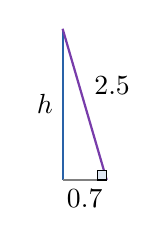
\begin{tikzpicture}[scale=0.8]
  \coordinate (B) at (0,0);
  \coordinate (A) at (0,2.4);
  \coordinate (C) at (0.7,0);
  \draw[thick, mainblue] (B)--(A);
  \draw[thick, gray] (B)--(C);
  \draw[thick, apppurple] (A)--(C);
  \draw[fill=mainblue!15] (0.55,0) rectangle (0.7,0.15);
  \node[left] at (0,1.2) {$h$};
  \node[below] at (0.35,0) {$0.7$};
  \node[above right] at (0.35,1.2) {$2.5$};
\end{tikzpicture}
\end{center}

\[
h^2 + 0.7^2 = 2.5^2 \implies h^2 = 6.25 - 0.49 = 5.76 \implies h = 2.4 \text{ 米}
\]

\textbf{第二问：}顶端下滑 0.4 米，新高度 $= 2.4 - 0.4 = 2$ 米。设底端外滑 $x$ 米：
\[
2^2 + (0.7+x)^2 = 2.5^2
\]
\[
(0.7+x)^2 = 6.25 - 4 = 2.25 \implies 0.7+x = 1.5 \implies x = 0.8
\]
$\boxed{\text{顶端高 } 2.4 \text{ 米；底端外滑 } 0.8 \text{ 米}}$
\end{appbox}

% --- 应用2 ---
\begin{appbox}[【应用2】航行问题]
\textbf{题目：}一艘轮船从港口 $A$ 出发，向北偏东 $60°$ 方向航行 60 海里到达 $B$，再向北偏西 $30°$ 方向航行 80 海里到达 $C$。求 $A$、$C$ 之间的距离。

\vspace{6pt}
\textbf{解答：}

根据方向角，$\angle ABC = 60° + 30° = 90°$，所以 $\triangle ABC$ 是直角三角形。

\begin{center}
\begin{tikzpicture}[scale=0.6]
  \coordinate (A) at (0,0);
  \coordinate (B) at (3,5.2);
  \coordinate (C) at (-1,10.2);
  \draw[->, thick, gray] (A)--(0,6) node[above]{\small 北};
  \draw[thick, mainblue] (A)--(B) node[midway, left]{\small 60};
  \draw[thick, mainblue] (B)--(C) node[midway, left]{\small 80};
  \draw[thick, apppurple, dashed] (A)--(C);
  \draw[fill=mainblue!15] (0.4,4.8) -- (0.8,5.0) -- (0.4,5.4);
  \node[left] at (A) {$A$};
  \node[right] at (B) {$B$};
  \node[left] at (C) {$C$};
  \node[right] at (0.5,7) {$\angle ABC = 90°$};
\end{tikzpicture}
\end{center}

\[
AC = \sqrt{AB^2 + BC^2} = \sqrt{60^2 + 80^2} = \sqrt{3600+6400} = \sqrt{10000} = \boxed{100 \text{ 海里}}
\]
\end{appbox}

% --- 应用3 ---
\begin{appbox}[【应用3】旗杆测量]
\textbf{题目：}小明想知道旗杆的高度。他发现旗杆顶端的绳子垂到地面后还多出 1 米。当他把绳子拉直，底端刚好接触地面时，离旗杆底部恰好 5 米。旗杆有多高？

\vspace{6pt}
\textbf{解答：}

设旗杆高为 $h$ 米，则绳子长 $= h+1$ 米。
\begin{center}
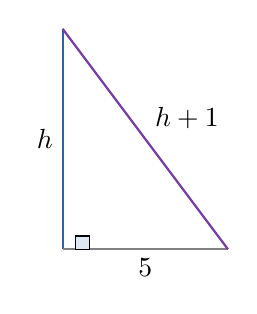
\begin{tikzpicture}[scale=0.7]
  \coordinate (B) at (0,0);
  \coordinate (A) at (0,4);
  \coordinate (C) at (3,0);
  \draw[thick, mainblue] (B)--(A);
  \draw[thick, gray] (B)--(C);
  \draw[thick, apppurple] (A)--(C);
  \draw[fill=mainblue!15] (0.24,0) rectangle (0.48,0.24);
  \node[left] at (0,2) {$h$};
  \node[below] at (1.5,0) {$5$};
  \node[above right] at (1.5,2) {$h+1$};
\end{tikzpicture}
\end{center}

\[
h^2 + 5^2 = (h+1)^2
\]
\[
h^2 + 25 = h^2 + 2h + 1 \implies 25 = 2h + 1 \implies 2h = 24
\]
\[
\boxed{h = 12 \text{ 米}}
\]
\end{appbox}

% --- 应用4 ---
\begin{appbox}[【应用4】面积与勾股定理]
\textbf{题目：}直角三角形两直角边之和为 14，斜边为 10，求三角形面积。

\vspace{6pt}
\textbf{解答：}

设两直角边为 $a$、$b$：
\[
\begin{cases} a + b = 14 \\ a^2 + b^2 = 100 \end{cases}
\]
由完全平方公式 $(a+b)^2 = a^2 + 2ab + b^2$：
\[
14^2 = 100 + 2ab \implies 196 = 100 + 2ab \implies ab = 48
\]
\[
S = \tfrac{1}{2}ab = \tfrac{1}{2} \times 48 = \boxed{24}
\]
\end{appbox}

\begin{tipbox}[技巧点拨]
不需要单独求 $a$ 和 $b$ 的值，利用\textbf{整体思想}直接求 $ab$ 即可。\\
关键公式：$(a+b)^2 = a^2 + b^2 + 2ab$
\end{tipbox}

% ============ 第四部分：课堂练习 ============
\section*{\textcolor{tipgreen}{四、课堂练习}}

\begin{enumerate}[leftmargin=2em, itemsep=8pt]
  \item 直角三角形两直角边为 9 和 12，求斜边。
  \item 直角三角形斜边为 17，一直角边为 8，求另一直角边。
  \item 三角形三边为 5,\ 12,\ 13，它是直角三角形吗？
  \item 一棵大树在风中折断，树的顶部落在离树根 8 米处，折断部分长 10 米。求大树原来的高度。
  \item 在平面直角坐标系中，点 $A(-1,2)$，$B(3,-2)$，求 $AB$ 的距离。
\end{enumerate}

\vspace{10pt}
\begin{knowledgebox}[参考答案]
\begin{enumerate}[leftmargin=2em, itemsep=4pt]
  \item $c = \sqrt{9^2+12^2} = \sqrt{81+144} = \sqrt{225} = \mathbf{15}$
  \item $b = \sqrt{17^2-8^2} = \sqrt{289-64} = \sqrt{225} = \mathbf{15}$
  \item 是。$5^2+12^2=25+144=169=13^2$，满足勾股定理，是直角三角形。\quad $\checkmark$
  \item 未折断部分高 $h = \sqrt{10^2-8^2} = \sqrt{36} = 6$ 米，原高 $= 6+8 = \mathbf{14}$ 米
  \item $d = \sqrt{(3-(-1))^2+(-2-2)^2} = \sqrt{16+16} = \mathbf{4\sqrt{2}}$
\end{enumerate}
\end{knowledgebox}

\vfill
\begin{center}
\small\textcolor{gray}{本讲义仅供教学参考，例题可根据学生水平调整难度。}
\end{center}

\end{document}
